\documentclass{report}
\usepackage[utf8]{inputenc}
\usepackage[T1]{fontenc}
\usepackage{amsmath, amsthm}
\usepackage{python}
\usepackage{listings}
\usepackage{float}
\usepackage{graphicx}
\usepackage{subcaption}
\usepackage{amssymb}
\usepackage{algorithm}
\usepackage{nccmath}
\usepackage{cite}

\newtheorem{theorem}{Theorem}[section]
\newtheorem{lemma}[theorem]{Lemma}
\newtheorem{proposition}[theorem]{Proposition}
\newtheorem{corollary}[theorem]{Corollary}
% % \theoremstyle{definition} %Makes def,ex and remark without italics
\newtheorem{definition}[theorem]{Definition}
\newtheorem{example}[theorem]{Example}
\newtheorem{remark}[theorem]{Remark}


\newcommand{\quoteswe}[1]{”#1”}
\newcommand{\quoteeng}[1]{“#1”}

\newcommand{\norm}[1]{\left\lVert#1\right\rVert}
\newcommand{\abs}[1]{\left| #1 \right|}
\newcommand{\inner}[2]{\left< #1 , #2 \right>}
\renewcommand{\Re}{\operatorname{Re}}
\renewcommand{\Im}{\operatorname{Im}}
\renewcommand{\phi}{\varphi}
\renewcommand{\Phi}{\varPhi}
\newcommand{\sgn}[1]{\operatorname{sgn} (#1)}
\newcommand{\csgn}[1]{\operatorname{csgn} (#1)}
\newcommand{\argmin}[1]{\underset{#1}{\arg\min}}
\newcommand{\Arg}{\operatorname{Arg}}
\renewcommand{\exp}[1]{\operatorname{e}^{#1}}
\newcommand{\expalt}{\operatorname{exp}}
\renewcommand{\i}{\mathrm{i}}
\newcommand{\id}{\mathrm{I}}
\newcommand{\T}{\mathrm{T}}
\newcommand{\coi}[2]{\left[#1, #2\right]}


\title{Relaxation Runge-Kutta Methods and Entropy Stability}
% \subtitle{}
\author{Thomas Renström}

\date{\today}

\begin{document}

\chapter{Introduction}

For certain simulations it is of utmost importance to use methods that follow conservation laws, making sure that the model stays true to physical laws. While there are already established methods for this, none of them are as well known or as simple to set up as the Runge-Kutta method. Not only is the simple modification suggested in the article by Ranocha et al. \cite{Ranocha_2020} both simple and cheap, as we shall see it is also accurate.

\chapter{Preliminaries}
\section{ODE}
    We consider a time-dependent ODE of the form
    \begin{align*}
        \frac{\text{d}}{\text{d}t} u(t) &= f(t, u(t)), \quad t \in (0, T)\\
        u(0) &= u^0
    \end{align*}
    for \(u \in \mathcal{H}\) being a real Hilbert space with the inner product \(\inner{\cdot}{\cdot}\), inducing the norm \(\norm{\cdot}\).


\section{Entropy}
    We denote by
    \[ \eta: \mathcal{H} \rightarrow \mathbb{R}\]
    a smooth convex function in time.
    We call this entropy, while in other application it might instead represent some other form of non-increasing quantity, e.g. energy or momentum.

    The change in entropy over time is given by
    \[\frac{\text{d}}{\text{d}t} \eta (u(t)) = \inner{\eta'(u(t))}{f(t, u(t))}.\]

    \vspace*{5mm}
    A entropy dissipative system will satisfy
    \[\inner{\eta'(u(t))}{f(t, u(t))} \leq 0, \quad \forall u \in \mathcal{H}, t \in [0, T],\]
    and a entropy conservative system will satisfy
    \[\inner{\eta'(u(t))}{f(t, u(t))} = 0, \quad \forall u \in \mathcal{H}, t \in [0, T].\]


\section{Classic Runge-Kutta}
    A general Runge-Kutta method with \(s\) stages is represented with the Butcher tableau
    \[\begin{array}{c|c}
        c & A\\
        \hline
        ~ & b^{\T}
    \end{array},\]
    with \(A \in \mathbb{R}^{s \times s}\) and \(b, c \in \mathbb{R}^s.\)

    \vspace*{7mm}
    \noindent
    The scheme of the method is
    \begin{align}
        y_i &= u^{n} + \Delta t\sum_{j=1}^{s} a_{i,j} f(t_n + c_j \Delta t, y_j), \quad i = 1,\ldots,s \label{Eq_RK_Stage} \\
        u^{n+1} &= u^{n} + \Delta t \sum_{i=1}^{s} b_i f(t_n + c_i \Delta t, y_i). \label{Eq_RK_Scheme}
    \end{align}
    where \(y_i\) are the stage values.

    \vspace*{7mm}
    \noindent
    For brevity we will use the notation
    \[f_i := f(t_n + c_i \Delta t, y_i), \qquad f_0 := f(t_n, u^n).\]


\chapter{Relaxation Runge-Kutta Methods}
\section{Relaxation Runge-Kutta}
    The basic idea of the Relaxed Runge-Kutta method is to introduce a scaling factor to the weights \(b_i\). We call this scaling factor \(\gamma_n \in \mathbb{R}\) and construct a new scheme
    \[u^{n+1}_{\gamma} = u^{n} + \gamma_n \Delta t \sum_{i=1}^{s} b_i f_i,\]
    with \(\gamma_n \in \mathbb{R}\).

    \vspace*{10mm}
    Relaxed Runge-Kutta, RRK, interprets \(u_{\gamma}^{n+1} \approx u(t_n + \gamma \Delta t)\). This means that using this method we will not be using a uniform step length and the number of steps might not be the same as with the regular RK method.

    \vspace*{5mm}
    The incremental direction technique, or IDT-method, interprets \(u_{\gamma}^{n+1} \approx u(t_n + \Delta t)\). This method retains the original step length, and takes as many steps to complete as the regular RK method it is based on.

    In a earlier work one of the authors proposed choosing \(\gamma_n\) such that
    \[ \frac{\norm{u^{n+1}_{\gamma}}^2 - \norm{u^{n}}^2}{2} = \gamma_n \Delta t \sum_{i=1}^{s} b_i \inner{y_i}{f_i} .\]

    In this article however the suggestion is to instead use \(\gamma_n\) fulfilling the condition
    \[  \eta (u^{n+1}_{\gamma}) - \eta (u^{n}) = \gamma \Delta t \sum_{i=1}^{s} b_i \inner{\eta'(y_i)}{f_i}.\]
    This is done by finding a root of
    \begin{equation}\label{Eq_r}
        r(\gamma) = \eta (u^{n} + \gamma_n \Delta t \sum_{i=1}^{s} b_i f_i) - \eta (u^{n}) - \gamma \Delta t \sum_{i=1}^{s} b_i \inner{\eta'(y_i)}{f_i}.
    \end{equation}

    The direction and entropy change
    \begin{align*}
        d^n &:= \sum^s_{i=1}b_if_i \\
        e   &:= \Delta t \sum^s_{i=1} b_i \inner{\eta'(y_i)}{f_i}
    \end{align*}
    can both be computed on the fly during the RK method. This reduces finding the root of \(r\) to just a scalar root finding problem.

    Note that since \(\eta\) is convex we have that \(r\) is convex in \(\gamma\).

    We note also that since
    \begin{equation}\label{Eq_r_at_0}
        r(0) = \eta (u^{n} + 0) - \eta (u^{n}) - 0 = 0
    \end{equation}
    \(r\) has a root at \(0\).

    Using a non-positive \(\gamma\) would not be feasible. A zero-valued \(\gamma\) would halt the scheme, while a negative \(\gamma\) would amount to steps backwards in time.

% \section{title}
%     Theorem 2.2
%

% \section{Existence of a solution}
% \section{Existence of a solution}
%     We know that \(r\) has one of the following forms
%     PICTURE
%     Now, in order to prove that \(r\) has a positive root we show that \(r(\gamma)\) is negative for small enough \(\gamma > 0\) and positive for large \(\gamma > 0\).
%


\section{Existence of a solution}
In order to show that \(r\) has a positive root we need two things. Firstly that \(r'\) is negative at the root \(\gamma = 0\) and that \(r'\) is positive at some point \(\gamma > 0\).

    \begin{lemma}
        Let a Runge-Kutta method be given such that \(\sum_{i=1}^{s}b_{i}a_{i,j}>0\). If \(n''(u^n)(f_0,f_0) > 0\) then \(r'(0)<0\) for sufficiently small \(\Delta t > 0\).
    \end{lemma}

    \vspace*{10mm}
    Note that \(\sum_{i=1}^{s}b_{i}a_{i,j}>0\) is a reasonable assumption,
    since \(\sum_{i=1}^{s}b_{i}a_{i,j}=1/2\) is a condition for second-order accuracy.

    % \begin{proof}
    %     By definition of \(r\) we have that
    %     \begin{align*}
    %         r'(0)   &= \eta'(u^n) \cdot \left(\Delta t \sum_{i=1}^{s}b_if_i\right) - \Delta t \sum_{i=1}^{s}b_i\inner{\eta'(y_i)}{f_i}\\
    %         &= -\Delta t^2 \sum_{i,j=1}^{s}b_ia_{i,j} \int_{0}^{1}\eta''\left(u^n + v\Delta t \sum_{k=1}^{s}a_{i,k}f_k\right)\left(f_i,f_j\right)\text{d}v.
    %     \end{align*}
    %     With Taylor expansions of \(f_i, f_j = f_0 + \mathcal{O}(\Delta t)\),
    %     \begin{align*}
    %         r'(0) &= -\Delta t^2 \sum_{i,j=1}^{s}b_ia_{i,j} \int_{0}^{1}\eta''\left(u^n + v\Delta t \sum_{k=1}^{s}a_{i,k}f_k\right)\left(f_0,f_0 \right)\text{d}v + \mathcal{O}(\Delta t^3)
    %     \end{align*}
    %     Thus, with the given assumptions, \(r'(0)<0\).
    % \end{proof}

    \begin{proof}
        By the definition of \(r(\gamma)\) in Equation~\ref{Eq_r},
        \begin{align*}
            \frac{dr}{d\gamma}  &= \eta'(u^n + \gamma \Delta t \sum_{i=1}^{s}b_if_i) \cdot \left(\Delta t \sum_{i=1}^{s}b_if_i\right) - \Delta t \sum_{i=1}^{s}b_i\inner{\eta'(y_i)}{f_i}.
        \end{align*}

        Evaluating \(r'(\gamma)\) at \(\gamma = 0\) we get
        \begin{align*}
            r'(0)   &= \eta'(u^n) \cdot \left(\Delta t \sum_{i=1}^{s}b_if_i\right) - \Delta t \sum_{i=1}^{s}b_i\inner{\eta'(y_i)}{f_i}\\
                    &= \Delta t \sum_{i=1}^{s}b_i \left( \inner{\eta'(u^n)}{f_i} - \inner{\eta'(y_i)}{f_i}\right) \\
                    &= -\Delta t \sum_{i=1}^{s}b_i \left( \inner{\eta'(y_i)}{f_i} - \inner{\eta'(u^n)}{f_i}\right).
        \end{align*}
        We expand \(y_i = u^n + \Delta t \sum_{j=1}^{s}a_{i,j}f_j\) as defined in Equation~\ref{Eq_RK_Stage} and get
        \begin{align*}
            r'(0) &= -\Delta t \sum_{i=1}^{s}b_i \left( \inner{\eta'\left(u^n + \Delta t \sum_{j=1}^{s}a_{i,j}f_j\right)}{f_i} - \inner{\eta'(u^n)}{f_i}\right).
        \end{align*}


        Then, by the fundamental theorem of calculus,
        \begin{align*}
            r'(0)   &= -\Delta t \sum_{i=1}^{s}b_i \int_{0}^{1}\eta''\left(u^n + v\Delta t \sum_{k=1}^{s}a_{i,k}f_k\right)\left(f_i,\Delta t \sum_{j=1}^{s}a_{i,j}f_j\right)\text{d}v \\
%                    &= -\Delta t^2 \sum_{i=1}^{s}b_i \int_{0}^{1}\eta''\left(u^n + \Delta t \sum_{k=1}^{s}a_{i,k}f_k\right)\left(f_i,\sum_{j=1}^{s}a_{i,j}f_j\right)\text{d}v \\
                    &= -\Delta t^2 \sum_{i,j=1}^{s}b_ia_{i,j} \int_{0}^{1}\eta''\left(u^n + v\Delta t \sum_{k=1}^{s}a_{i,k}f_k\right)\left(f_i,f_j\right)\text{d}v.
        \end{align*}
        With Taylor expansions of \(f_i, f_j = f_0 + \mathcal{O}(\Delta t)\),
        \begin{align*}
            r'(0)   &= -\Delta t^2 \sum_{i,j=1}^{s}b_ia_{i,j} \int_{0}^{1}\eta''\left(u^n + v\Delta t \sum_{k=1}^{s}a_{i,k}f_k\right)\left(f_0,f_0 + \mathcal{O}(\Delta t)\right)\text{d}v\\
                    &= -\Delta t^2 \sum_{i,j=1}^{s}b_ia_{i,j} \int_{0}^{1}\eta''\left(u^n + v\Delta t \sum_{k=1}^{s}a_{i,k}f_k\right)\left(f_0,f_0 \right)\text{d}v + \mathcal{O}(\Delta t^3)
        \end{align*}
        Thus, with the given assumptions, \(r'(0)<0\).
    \end{proof}


    \begin{lemma}
        Let a Runge-Kutta method be given such that \(\sum_{i,j=1}^{s}b_{i}(a_{i,j} - b_j)<0\). If \(\eta''(u^n)(f_0,f_0) > 0\) then \(r'(1)>0\) for sufficiently small \(\Delta t > 0\).
    \end{lemma}

    \vspace*{10mm}
    Note that the assumption \(\sum_{i,j=1}^{s}b_{i}(a_{i,j} - b_j)<0\) is reasonable. Since \(\sum_{i,j=1}^{s}b_{i}b_j = 1\) and \(\sum_{i=1}^{s}b_{i}a_{i,j}=1/2\) is a condition for second-order accuracy we have that \(\sum_{i,j=1}^{s}b_{i}(a_{i,j} - b_j)=-1/2\)

    \begin{proof}
        By the definition of \(r(\gamma)\) in Equation~\ref{Eq_r},
        \begin{align*}
            \frac{dr}{d\gamma}  &= \eta'(u^n + \gamma \Delta t \sum_{i=1}^{s}b_if_i) \cdot \left(\Delta t \sum_{i=1}^{s}b_if_i\right) - \Delta t \sum_{i=1}^{s}b_i\inner{\eta'(y_i)}{f_i}.
        \end{align*}

        Evaluating \(r'(\gamma)\) at \(\gamma = 1\) we get
        \begin{align*}
            r'(1)   &= \eta'(u^n + \Delta t \sum_{j=1}^{s}b_jf_j) \cdot \left(\Delta t \sum_{i=1}^{s}b_if_i\right) - \Delta t \sum_{i=1}^{s}b_i\inner{\eta'(y_i)}{f_i} \\
                    &= \Delta t \sum_{i=1}^{s}b_i \left( \inner{\eta'(u^n + \Delta t \sum_{j=1}^{s}b_jf_j)}{f_i} - \inner{\eta'(y_i)}{f_i} \right) \\
                    &= -\Delta t \sum_{i=1}^{s}b_i \left( \inner{\eta'(y_i)}{f_i} - \inner{\eta'(u^n + \Delta t \sum_{j=1}^{s}b_jf_j)}{f_i} \right)
        \end{align*}

        Expanding \(y_i = u^n + \Delta t \sum_{j=1}^{s}a_{i,j}f_j\) as defined in Equation~\ref{Eq_RK_Stage} we get
        \begin{equation*}
            r'(1) = -\Delta t \sum_{i=1}^{s}b_i \left( \inner{\eta'(u^n + \Delta t \sum_{j=1}^{s}a_{i,j}f_j)}{f_i} - \inner{\eta'(u^n + \Delta t \sum_{j=1}^{s}b_jf_j)}{f_i} \right).
        \end{equation*}

        We then make substitutions according to Equation~\ref{Eq_RK_Scheme}, \(u^{n+1} = u^n + \Delta t \sum_{j=1}^{s}b_jf_j\),
        \begin{equation*}
            r'(1) = -\Delta t \sum_{i=1}^{s}b_i \left(\inner{\eta'\left(u^{n+1} + \Delta t \sum_{j=1}^s \left(a_{i,j}-b_j\right)f_j\right)}{f_i} - \inner{\eta'(u^{n+1})}{f_i} \right).
        \end{equation*}

        Then, by the fundamental theorem of calculus,
        \begin{equation*}
            r'(1) = -\Delta t \sum_{i=1}^{s}b_i \int_{0}^{1} \eta'' \left(u^{n+1} + \Delta t \sum_{k=1}^s \left(a_{i,k}-b_k\right)f_k\right)\left(f_i,\Delta t \sum_{j=1}^s \left(a_{i,j}-b_j\right)f_j\right) \text{d}v
        \end{equation*}
        \begin{equation*}
            r'(1) = -\Delta t^2 \sum_{i,j=1}^{s}b_i\left(a_{i,j}-b_j\right) \int_{0}^{1} \eta'' \left(u^{n+1} + \Delta t \sum_{k=1}^s \left(a_{i,k}-b_k\right)f_k\right)\left(f_i,f_j\right) \text{d}v
        \end{equation*}

        With Taylor expansions of \(f_i, f_j = f_0 + \mathcal{O}(\Delta t)\),
        \begin{equation*}
            r'(1) = -\Delta t^2 \sum_{i,j=1}^{s}b_i\left(a_{i,j}-b_j\right) \int_{0}^{1} \eta'' \left(u^{n+1} + \Delta t \sum_{k=1}^s \left(a_{i,k}-b_k\right)f_k\right) \left(f_0,f_0+\mathcal{O}(\Delta t)\right) \text{d}v
        \end{equation*}
        \begin{equation*}
            r'(1) = -\Delta t^2 \sum_{i,j=1}^{s}b_i\left(a_{i,j}-b_j\right) \int_{0}^{1} \eta'' \left(u^{n+1} + \Delta t \sum_{k=1}^s \left(a_{i,k}-b_k\right)f_k\right) \left(f_0,f_0\right) \text{d}v+\mathcal{O}(\Delta t^3)
        \end{equation*}
        Thus, with the given assumptions, \(r'(1)>0\).
    \end{proof}

    \begin{theorem}
        Assume that the Runge-Kutta method satisfies \(\sum_{i,j=1}^{s} b_ia_{i,j}> 0\) and \(\sum_{i,j=1}^{s} b_i(a_{i,j}-b_j) < 0\). If \(\eta''(u^n)(f_0,f_0) > 0\) then r has a positive root for sufficiently small \(\Delta t > 0\).
    \end{theorem}
    \begin{proof}
        Since \(r(0)=0\) and \(r'(0) < 0\) we have that \(r(\gamma)<0\) for small \(\gamma > 0\). Because \(r'(1)>0\) and \(r\) is convex we have that \(r'\) is monotone. Thus, there must be a positive root of \(r\).
    \end{proof}


\section{Accuracy}
    \begin{theorem}
        Let a given RK-method be of order \(p\). Consider the IDT and RRK methods based on them and suppose that \(\gamma_n = 1 + \mathcal{O}(\Delta t^{p-1})\), then
        \begin{enumerate}
            \item The IDT method interpreting \(u_{\gamma}^{n+1} \approx u(t_n + \Delta t)\) has order \(p-1\).
            \item The RRK method interpreting \(u_{\gamma}^{n+1} \approx u(t_n + \gamma \Delta t)\) has order \(p\).
        \end{enumerate}
    \end{theorem}

    \begin{theorem}
        Let \(\mathcal{W}\) be a Banach space, \(\Phi: \left[0,T\right]\times \mathcal{H} \rightarrow \mathcal{W}\) a smooth function and \(b_i, c_i\) coefficients of a Runge-Kutta method of order \(p\). Then
        \[\sum_{i=1}^s b_i\Phi(t_n + c_i \Delta t, y_i) = \sum_{i=1}^{s}b_i\Phi(t_n + c_i \Delta t, u(t_n + c_i \Delta t)) + \mathcal{O}(\Delta t^p).\]
    \end{theorem}
    \begin{corollary}
        If \(\eta\) is smooth and the given Runge-Kutta method is \(p\)-order accurate, \(r(\gamma = 1) = \mathcal{O}(\Delta t^{p+1})\).
    \end{corollary}


    \begin{theorem}
        Assume there exists a positive root \(\gamma_n\) of \(r\). Consider the IDT/RRK methods based on a given Runge-Kutta method that is \(p\)-order accurate. Then
        \begin{enumerate}
            \item The IDT method interpreting \(u_{\gamma}^{n+1} \approx u(t_n + \Delta t)\) has order \(p-1\).
            \item The RRK method interpreting \(u_{\gamma}^{n+1} \approx u(t_n + \gamma \Delta t)\) has order \(p\).
        \end{enumerate}
    \end{theorem}
    \begin{proof}
        We have that \(r(1) = \mathcal{O}(\Delta t^{p+1})\) and \(r'(1)=c\Delta t^2 + \mathcal{O}(\Delta t^{3})\) for some \(c>0\). Thus there is a root \(\gamma_n = 1 + \mathcal{O}(\Delta t^{p-1})\) of \(r\). Applying to earlier theorem yield the desired result.
    \end{proof}


\chapter{Numerical Examples}

    Since the stepsize of RRK is unknown apriori, the last step of the method is always made using the ordinary RK method. This was applied to the IDT methods as well, although not necessary.
    Because of this we are in our convergence studies regarding the second to last value instead of the last.

    \vspace*{5mm}
    We are studying the effects of values of \(\Delta t\) close to \(1\) in the examples. These are not reasonable choices for \(\Delta t\), as the roots of \(r\) become less predictable. For the scalar root finding the method \texttt{scipy.optimize.root\_scalar} was used within the hardcoded range \( \left[0.5,2\right] \) was used.

    \vspace*{5mm}
    Note that fewer RK-methods were used for Problem 1 than in Problem 2. This is because the higher order Runge-Kutta methods resulted in an error from the method \texttt{isClose} used somewhere in \texttt{Assimulo}, a library of solvers that ours were written to inherit from.



\section{Problem 1 - Conserved exponential entropy}
    First we consider the system

    \[\frac{\text{d}}{\text{d}t}
    \begin{bmatrix}
        u_1(t)\\
        u_2(t)
    \end{bmatrix} =
    \begin{bmatrix}
        -\expalt(u_2(t))\\
        \expalt(u_1(t))
    \end{bmatrix}, \qquad u^0 =
    \begin{bmatrix}
        1\\
        0.5
    \end{bmatrix},
    \]
    with exponential entropy
    \[\eta(u) = \expalt(u_1) + \expalt(u_2), \qquad \eta'(u) =
    \begin{bmatrix}
        \expalt(u_1)\\
        \expalt(u_2)
    \end{bmatrix},
    \]
    and analytic solution
    \[u(t) = \left(\log\left(\frac{\exp{} + \exp{3/2}}{\sqrt{\exp{}} + \exp{(\sqrt{\exp{}}+\exp{})t}}\right), \log\left(\frac{\exp{(\sqrt{\exp{}}+\exp{})t}(\sqrt{\exp{}}+\exp{})}{\sqrt{\exp{}} + \exp{(\sqrt{\exp{}}+\exp{})t}}\right)\right)^{\T}.\]

    \begin{figure}[H]
        \centering
        \subfloat[\(r(\gamma)\) for SSPRK(3,3)\label{Fig1a}]{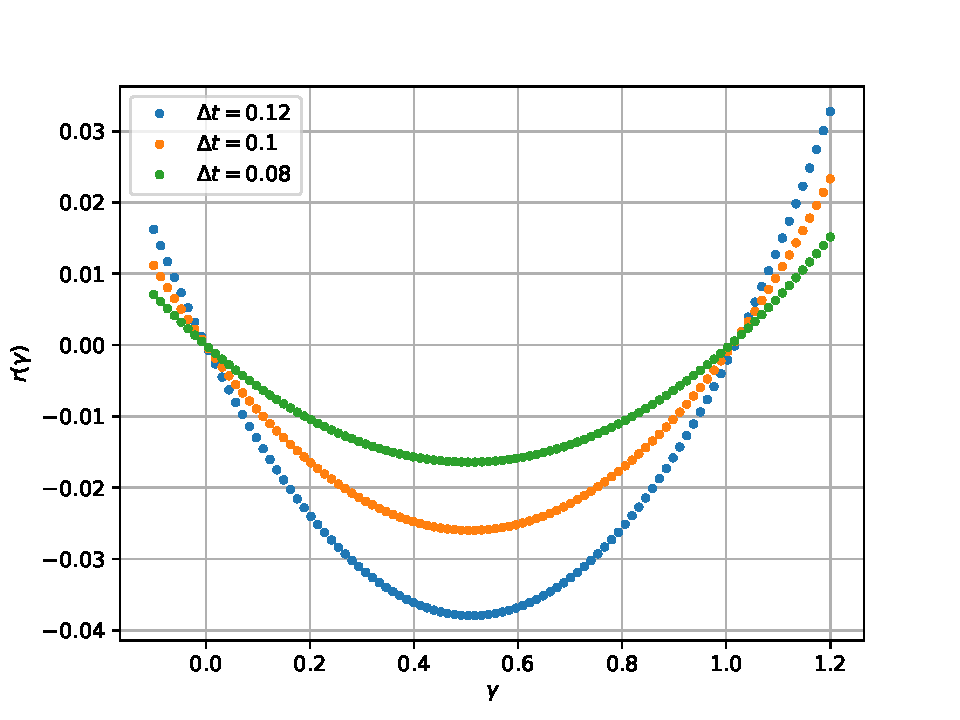
\includegraphics[width=0.50\textwidth]{figs/P1_r_of_gamma.pdf}}\hfill
        \subfloat[\(\left|r(\gamma = 1)\right|\) for some RK methods\label{Fig1b}] {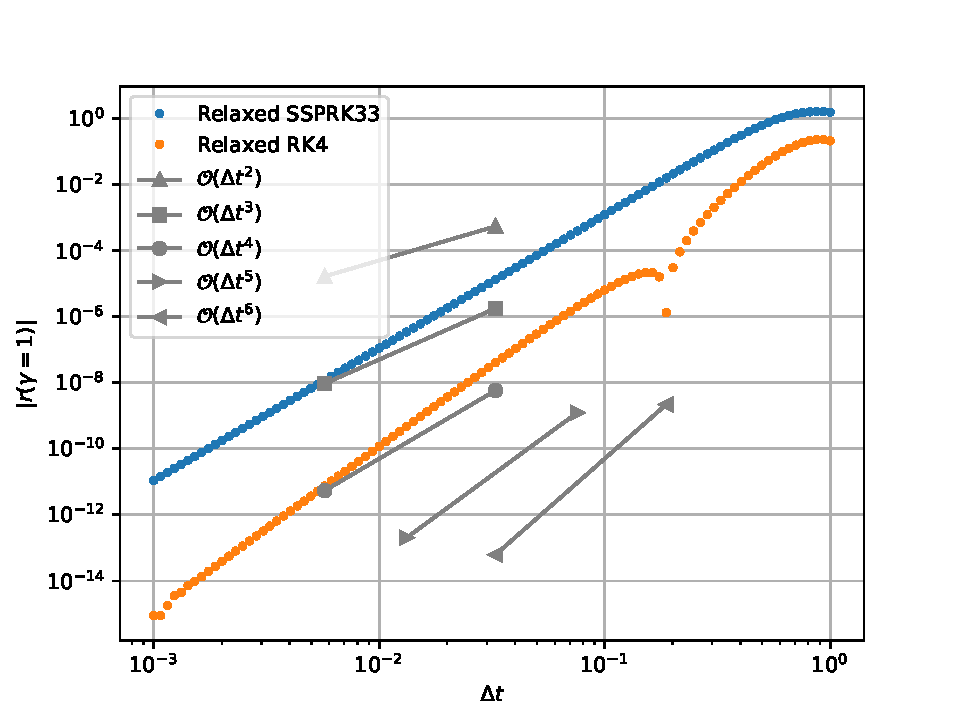
\includegraphics[width=0.50\textwidth]{figs/P1_r_at_1.pdf}}\hfill
        \caption{Numerical results for \(r\) at the first time step of problem 1.} \label{Fig1}
    \end{figure}

    \begin{figure}[H]
        \centering
        \subfloat[Classic methods\label{Fig2a}]{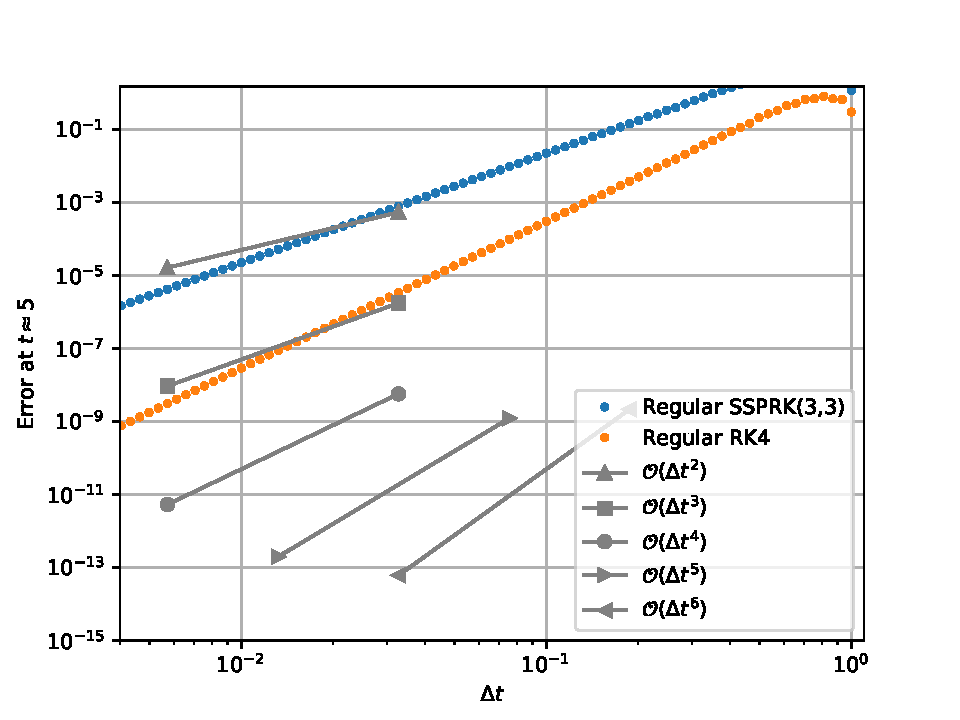
\includegraphics[width=0.33\textwidth]{figs/P1_Regular_RK4.pdf}}\hfill
        \subfloat[RRK Methods\label{Fig2b}] {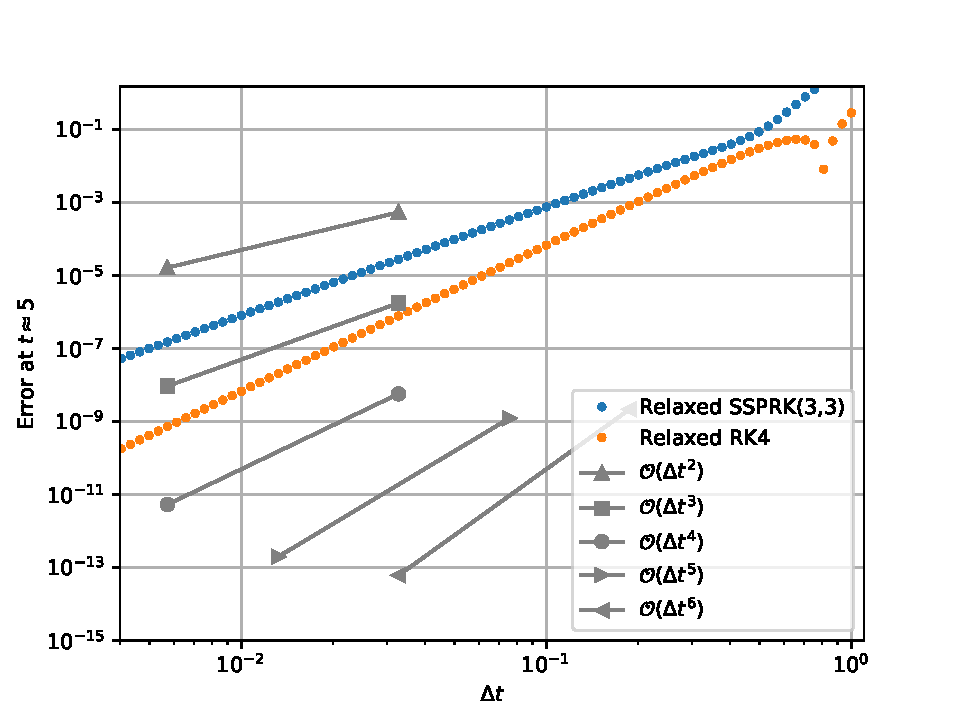
\includegraphics[width=0.33\textwidth]{figs/P1_Relaxed_RK4.pdf}}\hfill
        \subfloat[IDT methods\label{Fig2c}] {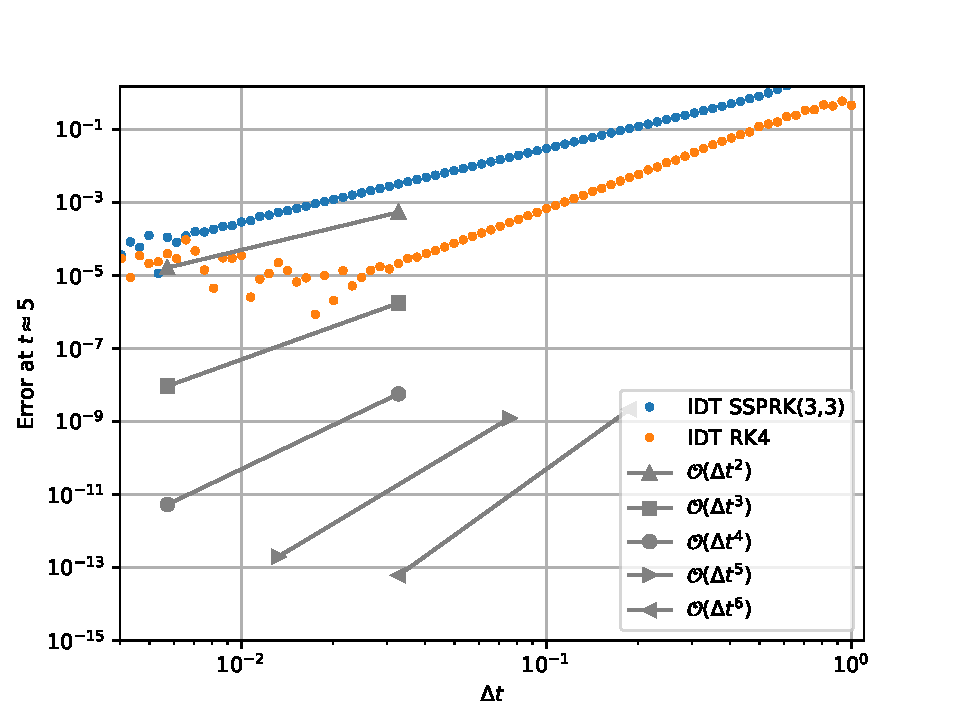
\includegraphics[width=0.33\textwidth]{figs/P1_IDT_RK4.pdf}}\hfill
        \caption{Convergence study for problem 1.} \label{Fig2}
    \end{figure}

    \begin{figure}[H]
        \centering
        \subfloat[SSPK(3,3)\label{Fig10a}]{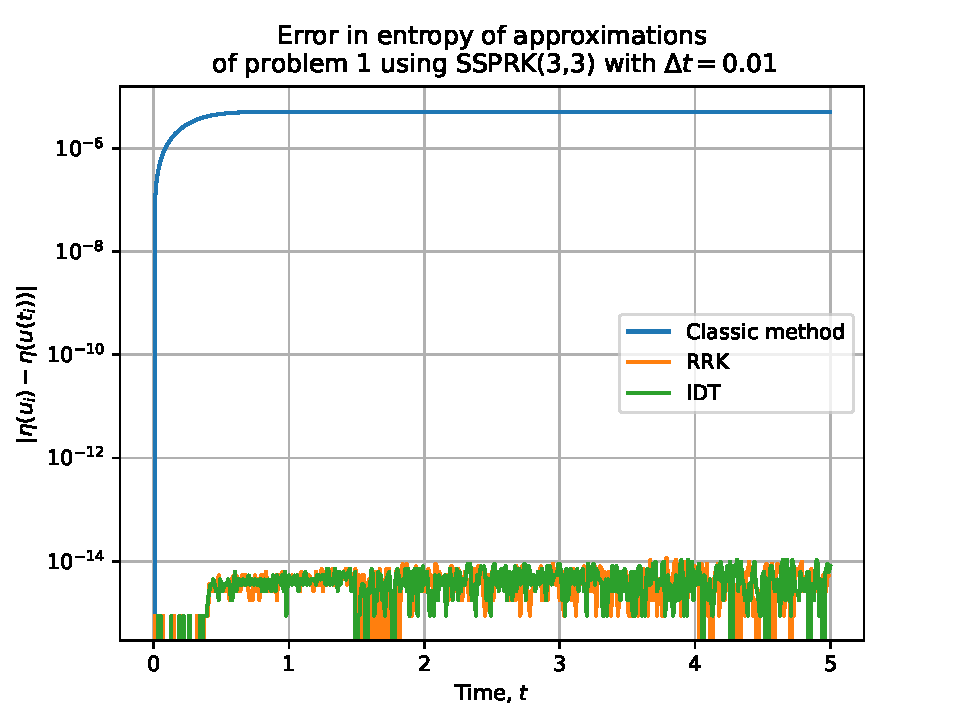
\includegraphics[width=0.5\textwidth]{figs/P1_eta_error_SSPRK33.pdf}}\hfill
        \subfloat[RK(4,4)\label{Fig10b}] {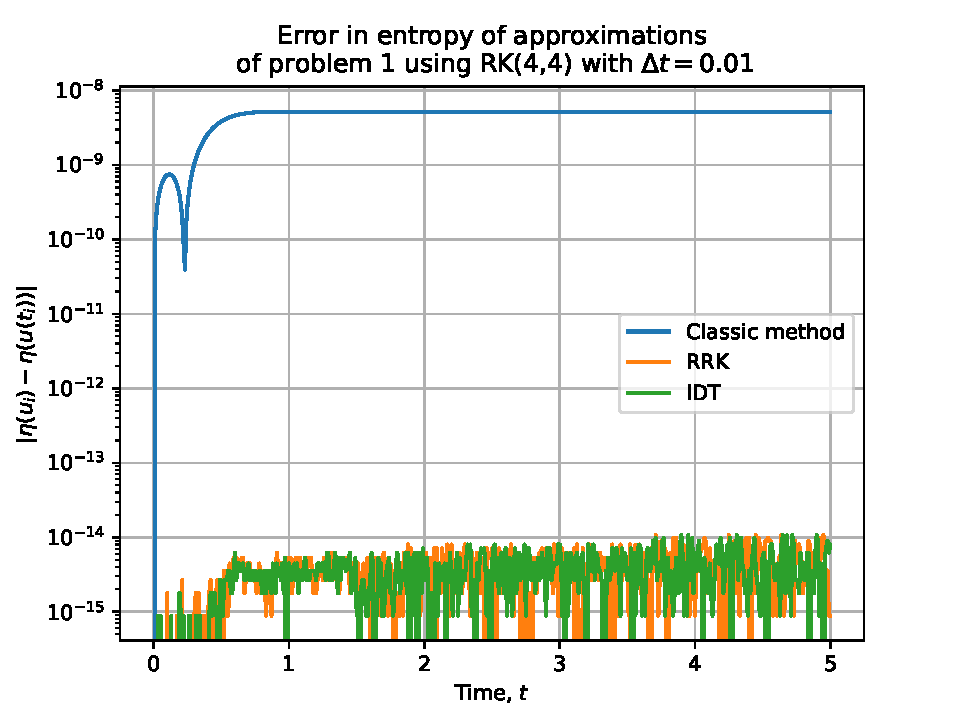
\includegraphics[width=0.5\textwidth]{figs/P1_eta_error_RK44.pdf}}\hfill
        \caption{Error of entropy for problem 1.}\label{Fig10}
    \end{figure}


\section{Problem 2 - Dissipated exponential entropy}
    Consider the ODE
    \[\frac{\text{d}}{\text{d}t} u(t) = -\expalt(u(t)), \qquad u^0 = 0.5,\]
    with the exponential entropy
    \[\eta(u) = \expalt(u), \qquad \eta'(u) = \expalt(u),\]
    and analytical solution
    \[u(t) = -\log(\exp{-1/2}+t).\]

    \begin{figure}[H]
        \centering
        \subfloat[\(r(\gamma)\) for SSPRK(3,3)\label{Fig3a}]{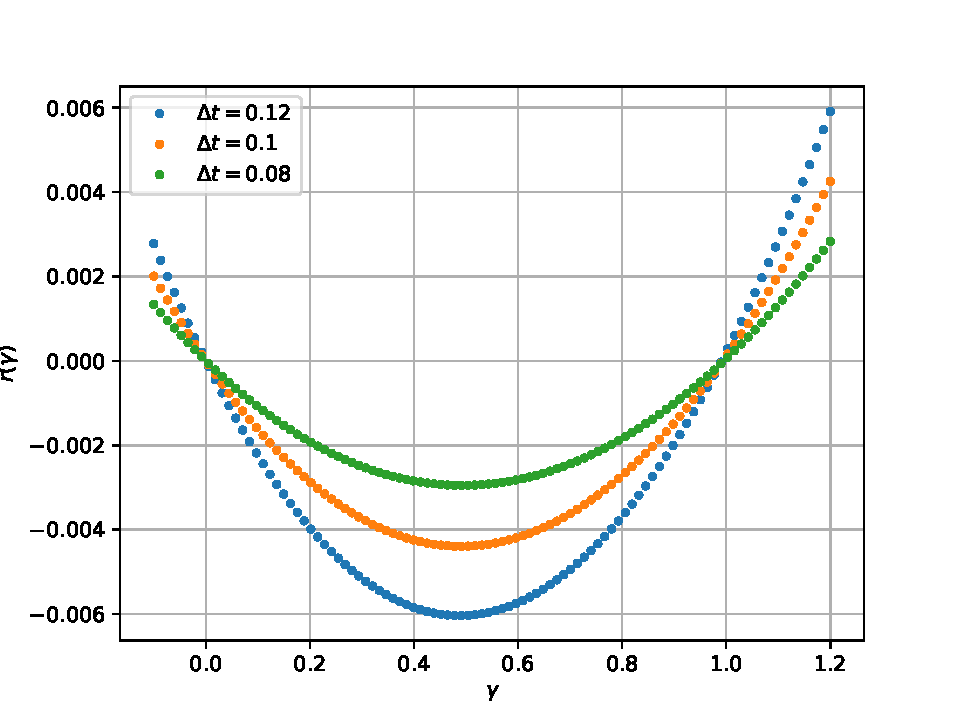
\includegraphics[width=0.48\textwidth]{figs/P2_r_of_gamma.pdf}}\hfill
        \subfloat[\(\left|r(\gamma = 1)\right|\) for some RK methods\label{Fig3b}] {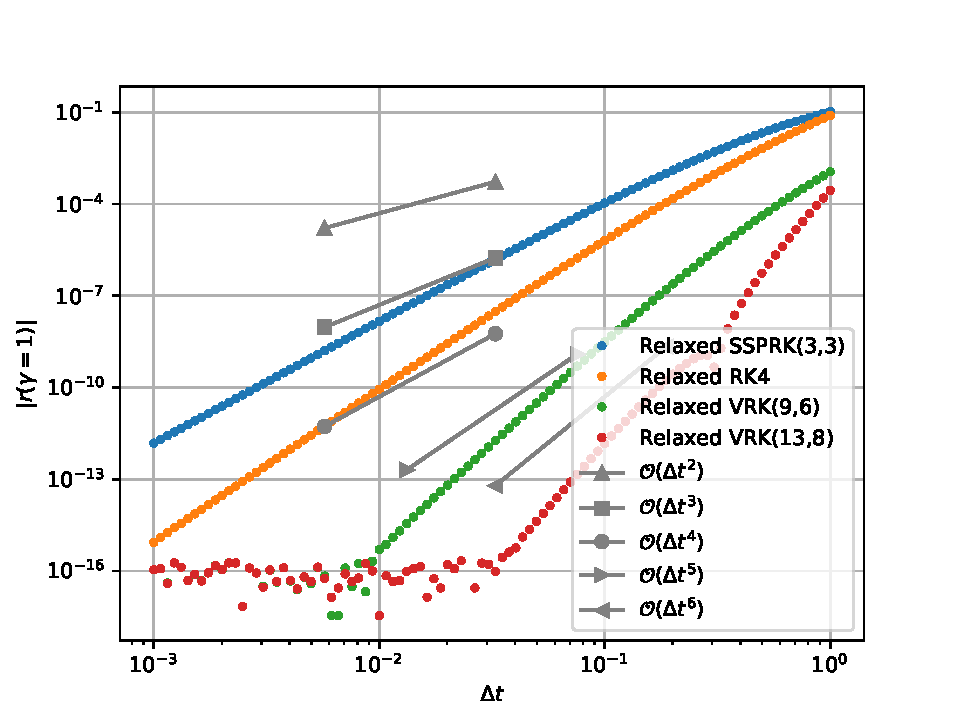
\includegraphics[width=0.48\textwidth]{figs/P2_r_at_1.pdf}}\hfill
        \caption{Numerical results for \(r\) at the first time step of problem 2.} \label{Fig3}
    \end{figure}

    \begin{figure}[H]
        \centering
        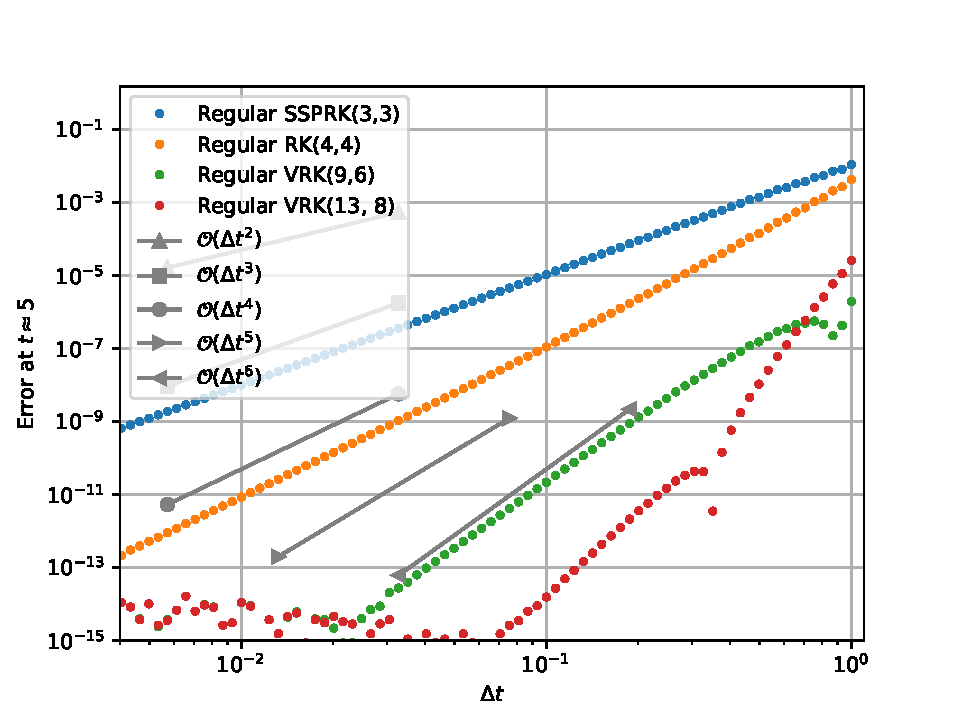
\includegraphics[width=0.95\textwidth]{figs/P2_Regular_RK4.pdf}
        \caption{Convergence study for problem 2, classic methods.}
        \label{Fig4a}
    \end{figure}

    \begin{figure}[H]
        \centering
        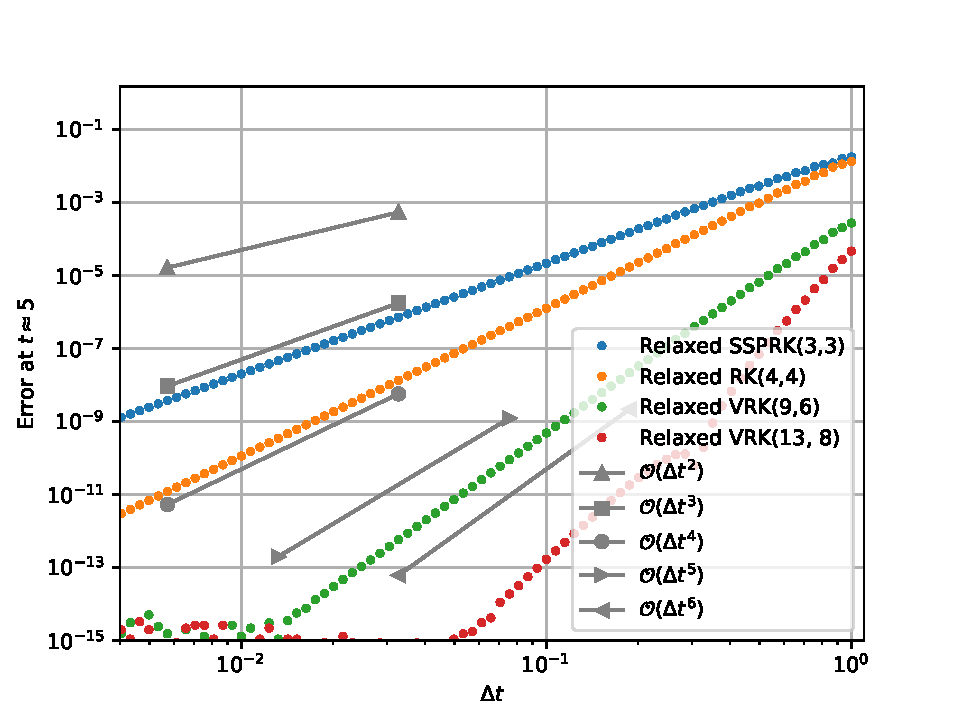
\includegraphics[width=0.95\textwidth]{figs/P2_Relaxed_RK4.pdf}
        \caption{Convergence study for problem 2, relaxed methods.}
        \label{Fig4b}
    \end{figure}

    \begin{figure}[H]
        \centering
        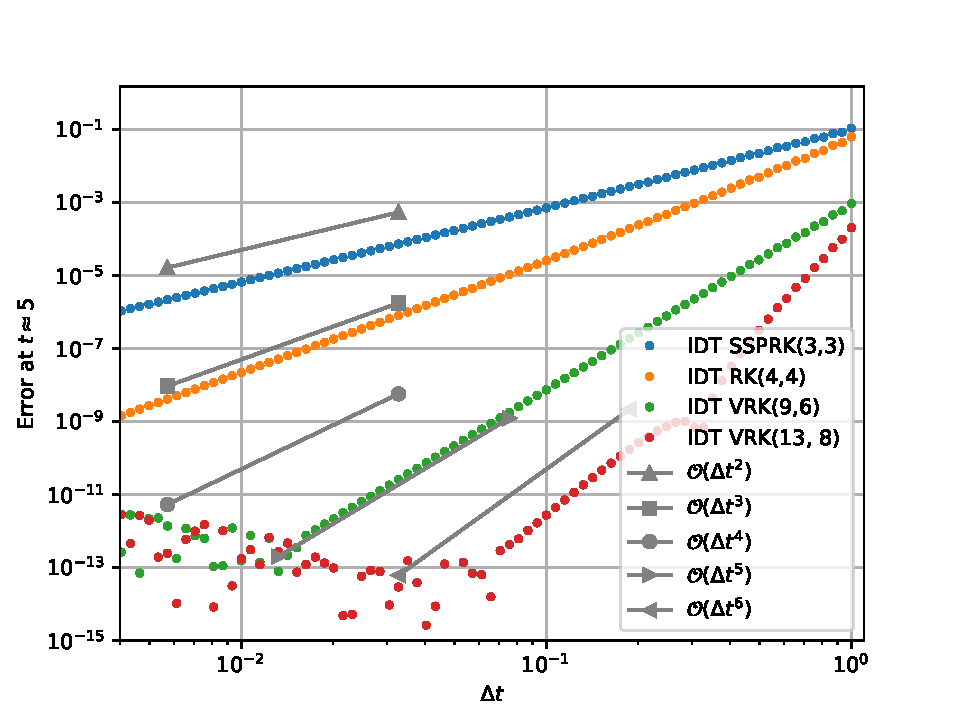
\includegraphics[width=0.95\textwidth]{figs/P2_IDT_RK4.pdf}
        \caption{Convergence study for problem 2, IDT methods.}
        \label{Fig4c}
    \end{figure}

    \begin{figure}[H]
        \centering
        \subfloat[SSPK(3,3)\label{Fig20a}]{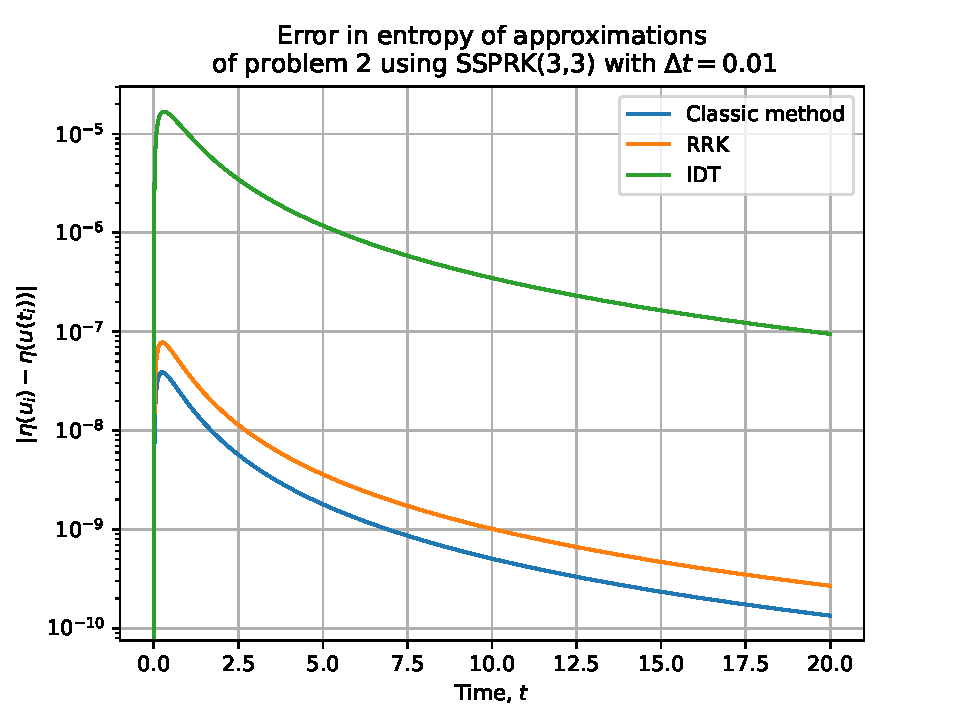
\includegraphics[width=0.5\textwidth]{figs/P2_eta_error_SSPRK33.pdf}}\hfill
        \subfloat[RK(4,4)\label{Fig20b}] {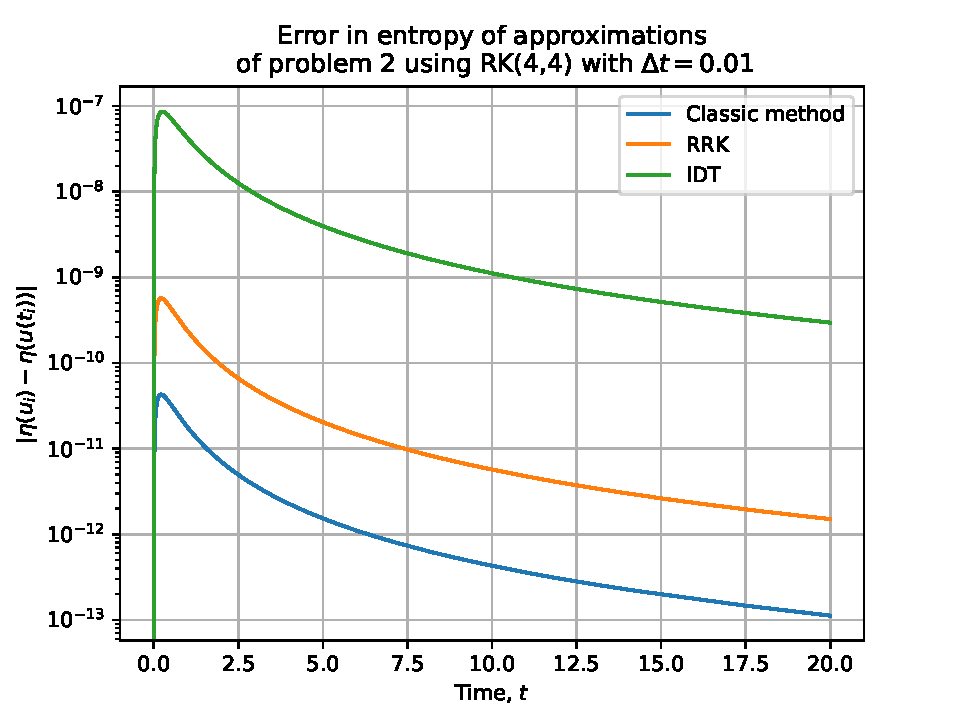
\includegraphics[width=0.5\textwidth]{figs/P2_eta_error_RK44.pdf}}\hfill\\
        \subfloat[VRK(9,6)\label{Fig20c}]{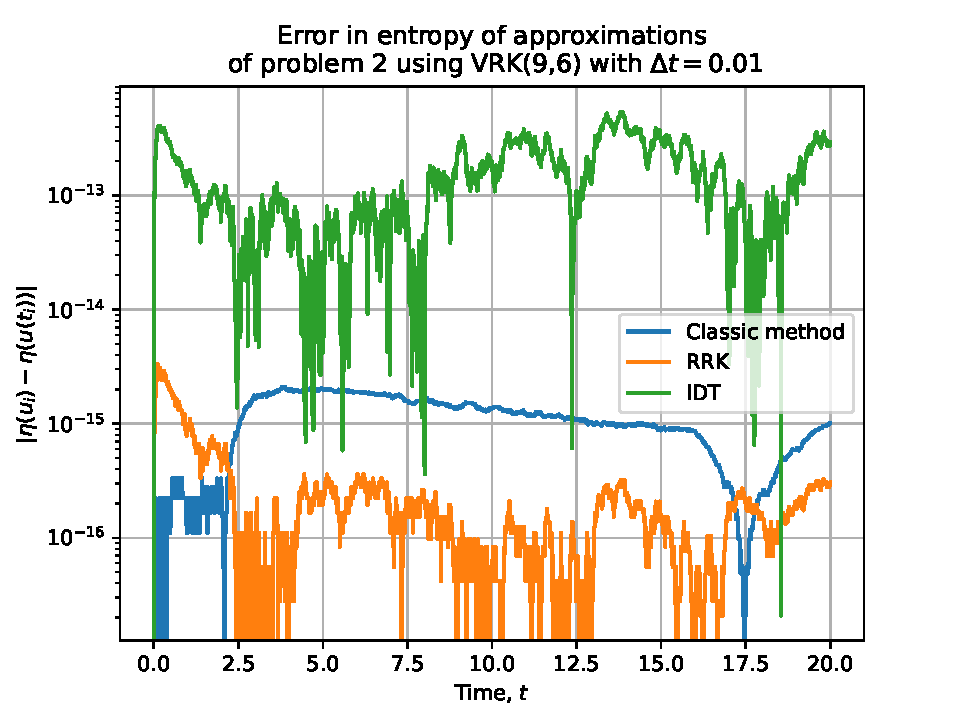
\includegraphics[width=0.5\textwidth]{figs/P2_eta_error_VRK96.pdf}}\hfill
        \subfloat[VRK(13,8)\label{Fig20d}] {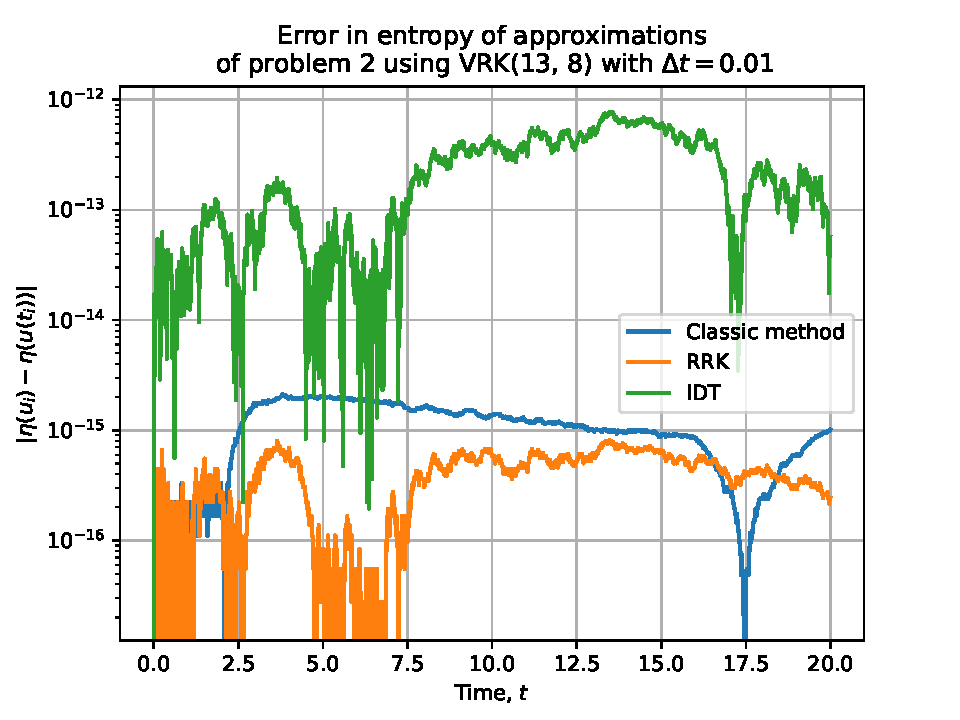
\includegraphics[width=0.5\textwidth]{figs/P2_eta_error_VRK138.pdf}}\hfill
        \caption{Error of entropy for problem 2.}\label{Fig20}
    \end{figure}


\chapter{Conclusion}
    \begin{itemize}
        \item Simple
        \item Cheap
        \item Physically correct
        \item Requires \(\eta\)
    \end{itemize}

One drawback is that the method requires prior knowledge of \(\eta\). This is however a reasonable assumption as someone interested in conserving the entropy of their simulation should have some insight into the entropy of their problem.
% However as a fallback a choice of \(\gamma_n\) satisfying
% \[ \frac{1}{2} \norm{u^{n+1}_{\gamma}}^2 - \frac{1}{2}\norm{u^{n}}^2 = \gamma_n \Delta t \sum_{i=1}^{s}b_i\inner{y_i}{f_i}\]
% as suggested by Ketcheson in \cite{ketcheson2019relaxation} could be used.

\bibliography{refs}{}
\bibliographystyle{plain}

\end{document}